\documentclass[11pt,compress,t,notes=noshow, xcolor=table]{beamer}
\usepackage[]{graphicx}\usepackage[]{color}
% maxwidth is the original width if it is less than linewidth
% otherwise use linewidth (to make sure the graphics do not exceed the margin)
\makeatletter
\def\maxwidth{ %
  \ifdim\Gin@nat@width>\linewidth
    \linewidth
  \else
    \Gin@nat@width
  \fi
}
\makeatother

\definecolor{fgcolor}{rgb}{0.345, 0.345, 0.345}
\newcommand{\hlnum}[1]{\textcolor[rgb]{0.686,0.059,0.569}{#1}}%
\newcommand{\hlstr}[1]{\textcolor[rgb]{0.192,0.494,0.8}{#1}}%
\newcommand{\hlcom}[1]{\textcolor[rgb]{0.678,0.584,0.686}{\textit{#1}}}%
\newcommand{\hlopt}[1]{\textcolor[rgb]{0,0,0}{#1}}%
\newcommand{\hlstd}[1]{\textcolor[rgb]{0.345,0.345,0.345}{#1}}%
\newcommand{\hlkwa}[1]{\textcolor[rgb]{0.161,0.373,0.58}{\textbf{#1}}}%
\newcommand{\hlkwb}[1]{\textcolor[rgb]{0.69,0.353,0.396}{#1}}%
\newcommand{\hlkwc}[1]{\textcolor[rgb]{0.333,0.667,0.333}{#1}}%
\newcommand{\hlkwd}[1]{\textcolor[rgb]{0.737,0.353,0.396}{\textbf{#1}}}%
\let\hlipl\hlkwb

\usepackage{framed}
\makeatletter
\newenvironment{kframe}{%
 \def\at@end@of@kframe{}%
 \ifinner\ifhmode%
  \def\at@end@of@kframe{\end{minipage}}%
  \begin{minipage}{\columnwidth}%
 \fi\fi%
 \def\FrameCommand##1{\hskip\@totalleftmargin \hskip-\fboxsep
 \colorbox{shadecolor}{##1}\hskip-\fboxsep
     % There is no \\@totalrightmargin, so:
     \hskip-\linewidth \hskip-\@totalleftmargin \hskip\columnwidth}%
 \MakeFramed {\advance\hsize-\width
   \@totalleftmargin\z@ \linewidth\hsize
   \@setminipage}}%
 {\par\unskip\endMakeFramed%
 \at@end@of@kframe}
\makeatother

\definecolor{shadecolor}{rgb}{.97, .97, .97}
\definecolor{messagecolor}{rgb}{0, 0, 0}
\definecolor{warningcolor}{rgb}{1, 0, 1}
\definecolor{errorcolor}{rgb}{1, 0, 0}
\newenvironment{knitrout}{}{} % an empty environment to be redefined in TeX

\usepackage{alltt}
\newcommand{\SweaveOpts}[1]{}  % do not interfere with LaTeX
\newcommand{\SweaveInput}[1]{} % because they are not real TeX commands
\newcommand{\Sexpr}[1]{}       % will only be parsed by R



\usepackage[english]{babel}
\usepackage[utf8]{inputenc}

\usepackage{dsfont}
\usepackage{verbatim}
\usepackage{amsmath}
\usepackage{amsfonts}
\usepackage{bm}
\usepackage{csquotes}
\usepackage{multirow}
\usepackage{longtable}
\usepackage{booktabs}
\usepackage{enumerate}
\usepackage[absolute,overlay]{textpos}
\usepackage{psfrag}
\usepackage{algorithm}
\usepackage{algpseudocode}
\usepackage{eqnarray}
\usepackage{arydshln}
\usepackage{tabularx}
\usepackage{placeins}
\usepackage{tikz}
\usepackage{setspace}
\usepackage{colortbl}
\usepackage{mathtools}
\usepackage{wrapfig}
\usepackage{bm}
\usetikzlibrary{shapes,arrows,automata,positioning,calc,chains,trees, shadows}
\tikzset{
  %Define standard arrow tip
  >=stealth',
  %Define style for boxes
  punkt/.style={
    rectangle,
    rounded corners,
    draw=black, very thick,
    text width=6.5em,
    minimum height=2em,
    text centered},
  % Define arrow style
  pil/.style={
    ->,
    thick,
    shorten <=2pt,
    shorten >=2pt,}
}
\usepackage{subfig}


% Defines macros and environments

% basic latex stuff
\newcommand{\pkg}[1]{{\fontseries{b}\selectfont #1}} %fontstyle for R packages
\newcommand{\lz}{\vspace{0.5cm}} %vertical space
\newcommand{\dlz}{\vspace{1cm}} %double vertical space
\newcommand{\oneliner}[1] % Oneliner for important statements
{\begin{block}{}\begin{center}\begin{Large}#1\end{Large}\end{center}\end{block}}

% 
% basic latex stuff
\newcommand{\pkg}[1]{{\fontseries{b}\selectfont #1}} %fontstyle for R packages
\newcommand{\lz}{\vspace{0.5cm}} %vertical space
\newcommand{\dlz}{\vspace{1cm}} %double vertical space
\newcommand{\oneliner}[1] % Oneliner for important statements
{\begin{block}{}\begin{center}\begin{Large}#1\end{Large}\end{center}\end{block}}


%\usetheme{lmu-lecture}
\newcommand{\titlefigure}{figure/cart_tuning_balgos_2}
\newcommand{\learninggoals}{
\item Understand the idea of grid search
\item Understand the idea of random search
\item Be able to discuss advantages and disadvantages of the two methods}
\usepackage{../../style/lmu-lecture}

\let\code=\texttt
\let\proglang=\textsf

\setkeys{Gin}{width=0.9\textwidth}

\title{Introduction to Machine Learning}
% \author{Bernd Bischl, Christoph Molnar, Daniel Schalk, Fabian Scheipl}
\institute{\href{https://compstat-lmu.github.io/lecture_i2ml/}{compstat-lmu.github.io/lecture\_i2ml}}
\date{}

\setbeamertemplate{frametitle}{\expandafter\uppercase\expandafter\insertframetitle}



\begin{document}

% Load all R packages and set up knitr

% This file loads R packages, configures knitr options and sets preamble.Rnw as parent file
% IF YOU MODIFY THIS, PLZ ALSO MODIFY setup.Rmd ACCORDINGLY...








%! includes: tuning-tuningproblem

\lecturechapter{Hyperparameter Tuning - Basic Techniques}
\lecture{Introduction to Machine Learning}
\sloppy


\begin{vbframe}{Grid search}

\begin{itemize}
\item Simple technique which is still quite popular, tries all
HP combinations on a multi-dimensional discretized grid
\item For each hyperparameter a finite set of candidates is predefined
\item Then, we simply search all possible combinations in arbitrary order
\end{itemize}

\begin{footnotesize}
\begin{center}
Grid search over 10x10 points
\end{center}
\end{footnotesize}

\begin{knitrout}\scriptsize
\definecolor{shadecolor}{rgb}{0.969, 0.969, 0.969}\color{fgcolor}

{\centering 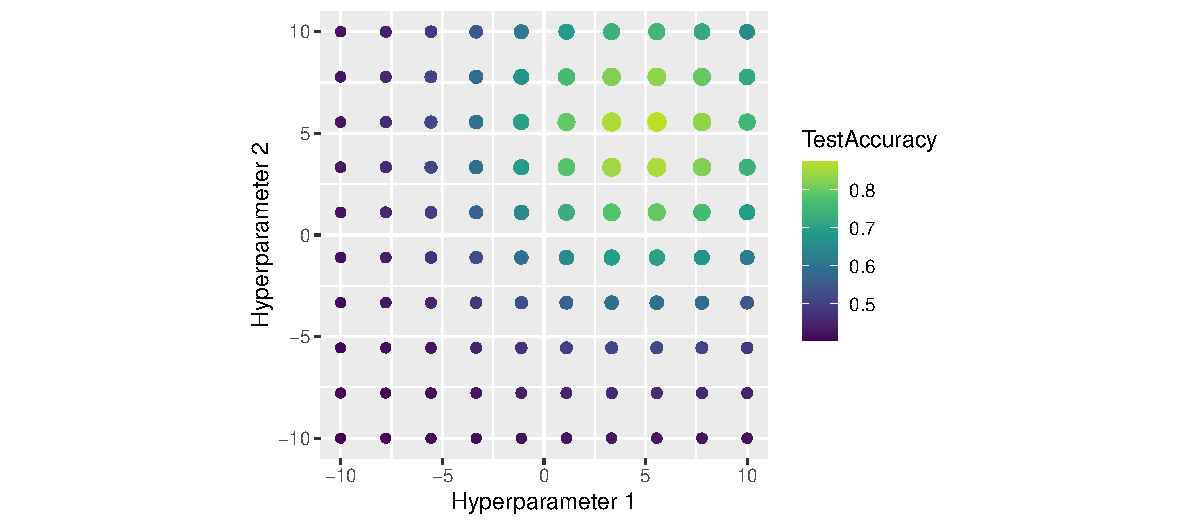
\includegraphics[width=0.95\textwidth]{figure/cart_tuning_balgos_1} 
}
% FIGURE SOURCE: fig-cart_tuning_balgos_1.R


\end{knitrout}


\framebreak

\begin{blocki}{Advantages}
\item Very easy to implement
\item All parameter types possible
\item Parallelizing computation is trivial
\end{blocki}

\begin{blocki}{Disadvantages}
\item  Scales badly: combinatorial explosion
\item  Inefficient: searches large irrelevant areas
\item  Arbitrary: which values / discretization?
\end{blocki}
\end{vbframe}


\begin{vbframe}{Random search}

\begin{itemize}
\item Small variation of grid search
\item Uniformly sample from the region-of-interest
\end{itemize}


\begin{footnotesize}
\begin{center}
Random search over 100 points
\end{center}
\end{footnotesize}

\begin{knitrout}\scriptsize
\definecolor{shadecolor}{rgb}{0.969, 0.969, 0.969}\color{fgcolor}

{\centering 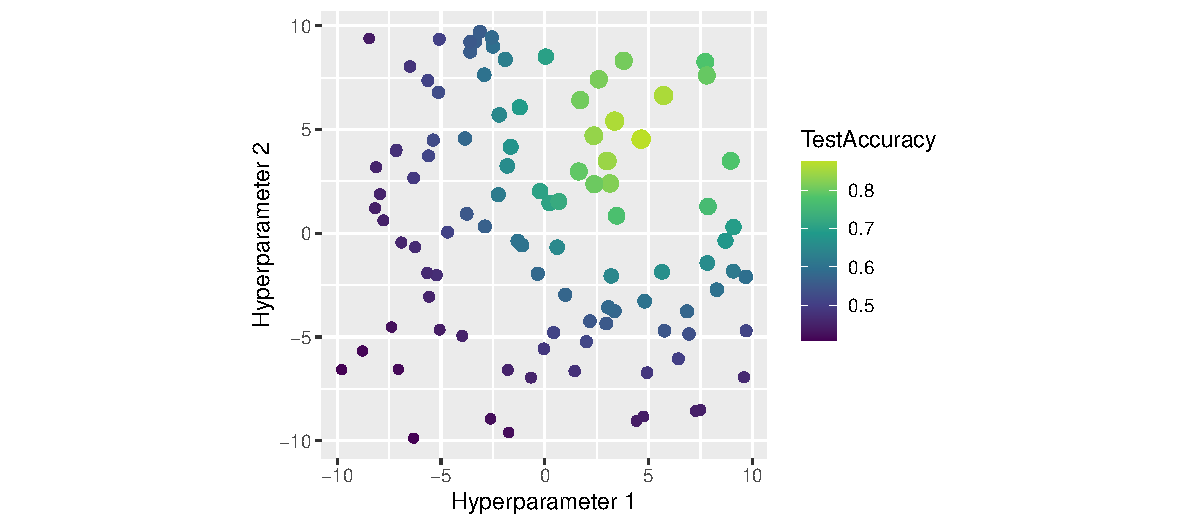
\includegraphics[width=0.95\textwidth]{figure/cart_tuning_balgos_2} 
}
% FIGURE SOURCE: fig-cart_tuning_balgos_1.R


\end{knitrout}

\framebreak

\begin{blocki}{Advantages}
\item Like grid search: very easy to implement, all parameter types possible, trivial parallelization
\item Anytime algorithm: can stop the search whenever our budget for computation is exhausted, or continue until we reach our performance goal.
\item No discretization: each individual parameter is tried with a different value every time
\end{blocki}
\vspace{-2ex}
\begin{blocki}{Disadvantages}
\item Inefficient: many evaluations in areas with low likelihood for improvement
\item Scales badly: high-dimensional hyperparameter spaces need \emph{lots} of samples to cover.
\end{blocki}
\end{vbframe}

\begin{vbframe}{Tuning Example}

Tuning random forest with random search and 5CV on the \texttt{sonar} data set for AUC:

\begin{footnotesize}
\begin{center}
\begin{tabular}{|l|l|l|l}
Hyperparameter          &  Type     & Min & Max \\
\hline
\texttt{num.trees}     & integer  & 3 & 500 \\
\texttt{mtry}          & integer  & 5 & 50  \\
\texttt{min.node.size} & integer  & 10 & 100\\
\end{tabular}
\end{center}
\end{footnotesize}

\begin{knitrout}\scriptsize
\definecolor{shadecolor}{rgb}{0.969, 0.969, 0.969}\color{fgcolor}

{\centering \includegraphics[width=0.95\textwidth]{figure/cart_tuning_balgos_3}
}
%FIGURE SOURCE: fig-cart_tuning_balgos_2


\end{knitrout}

\end{vbframe}

\endlecture
\end{document}
